\documentclass{article}

\textwidth=6.5in
\textheight=8.5in
\voffset=-54pt
\oddsidemargin=0in
\evensidemargin=0in
\setlength{\parskip}{8pt}
\setlength{\parindent}{0pt}

\usepackage{amsmath, amssymb}
\usepackage{ifthen}

\usepackage[inline]{enumitem}
\setlist{topsep=0pt, parsep=8pt}

\usepackage[rgb,table]{xcolor}\convertcolorsUfalse
\usepackage{graphicx}

% change hyperref options
\PassOptionsToPackage{hyphens}{url}
\usepackage[bookmarks,colorlinks,linkcolor=black,citecolor=blue,pdfstartview=FitH,urlcolor=blue]{hyperref}
\hypersetup{pdfpagemode=UseNone}
\usepackage{bookmark}

\usepackage{graphicx}
\usepackage{multicol}
\usepackage{framed}
\usepackage{array}

\usepackage{icomma}

\usepackage{soul}

\usepackage{pgfplots}
\pgfplotsset{compat=1.18}  
\pgfplotscreateplotcyclelist{mycolor}{black, blue, red, green!70!black, magenta, purple, cyan, orange }  
\pgfplotsset{
  disabledatascaling,
  cycle list=tikzcolor, 
  axis lines=middle,
  every axis plot/.style={no marks, thick},
  every axis/.style={
    enlarge x limits=false,
    enlarge y limits=auto,
    xlabel style={at={(current axis.right of origin)},anchor=west},
    ylabel style={at={(current axis.above origin)},anchor=south},
    % extra x and y ticks for asymptotes
    extra x tick style={grid=major, grid style={dashed,black}},
    extra y tick style={grid=major, grid style={dashed,black}},
    /pgf/number format/1000 sep={},
  },    
  tick label style = {font=\footnotesize, fill=\currentbgcolor, inner sep=0pt},    
  xticklabel shift=1pt,    
  scaled ticks=false,
  scaled y ticks=false,
  unbounded coords=jump,
  samples=101,
  minor tick length=0,
  scatter/classes={
    open={mark=*,draw=black,fill=white, mark size=2, thin},
    closed={mark=*,draw=black,fill=black, mark size=2, thin}
  },
  width=3in,
}
\pgfplotsset{open/.style={only marks, mark=*, fill=white, thin, mark size=2}}
\pgfplotsset{closed/.style={only marks, mark=*, draw=black, fill=black,
    thin, mark size=2}}
\pgfplotsset{labeled/.style={nodes near coords, only marks, mark=*, draw=black, fill=black, thin, mark size=2, point meta=explicit symbolic}}

\newcommand{\axes}[1][]{
  \begin{tikzpicture}
    \begin{axis}[xtick=\empty, ytick=\empty, ymin=-2, ymax=2,
      xmin=-4.25, xmax=4.25, #1]
    \end{axis}
  \end{tikzpicture}
}
\usepackage{tikz}
\usetikzlibrary{
  matrix,%
  % enables the snake paths
  decorations.pathmorphing,%
  % enables bigger arrows
  decorations.markings,%
  decorations.pathreplacing,%
  decorations.text,%
  calc,%
  patterns,%
  shapes.geometric,%
  arrows,
  decorations.shapes,
  positioning,
  plotmarks,
  intersections
}
\tikzset{>=latex} % sets default arrow type in tikz
\tikzset{font=\normalsize}
\tikzset{mark size=1.5pt, mark options=thin}
\tikzset{pin distance=4pt,
  every pin edge/.style={<-, thin, shorten <= -2pt}}

\interfootnotelinepenalty=10000
\renewcommand{\thefootnote}{(\arabic{footnote})}

\usepackage{multirow, bigdelim}

% change to \usepackage[sols]{handout} to see solutions
\usepackage[]{handout}

\newcommand\iscurrentenumi[1]{%
  \ifthenelse{\equal{#1}{\theenumi}}{}{#1}}
\setenumerate[1]{ref=\#\arabic*}
\setenumerate[2]{ref=\protect\iscurrentenumi{\theenumi}(\alph*)}
\newcommand\enumiiprefix[2]{%
  \ifthenelse{{\equal{#1}{\theenumi}}\AND{\equal{#2}{(\alph{enumii})}}}{}{}%
  \ifthenelse{{\equal{#1}{\theenumi}}\AND{\NOT{\equal{#2}{(\alph{enumii})}}}}{#2}{}%
  \ifthenelse{\equal{#1}{\theenumi}}{}{#1#2}%
}
\setenumerate[3]{ref=\protect\enumiiprefix{\theenumi}{(\alph{enumii})}\roman*}

\newlength{\tipmargin}
\makeatletter

\renewenvironment{framed}{
  \setlength{\tipmargin}{\textwidth-\linewidth}
  \advance\@totalleftmargin-\tipmargin
  \def\FrameCommand{\hspace{\tipmargin}\fbox}%
  \advance\linewidth\tipmargin
  \MakeFramed {\advance\hsize-\width \FrameRestore}%
}
{\endMakeFramed}

\makeatother

\definecolor{purple}{rgb}{0.5,0,1.0}
\definecolor{hotpink}{rgb}{1, 0, 0.5}

\usepackage{fancyhdr}
\lhead{\textcolor{white}{This content is protected and may not be shared, uploaded, or distributed.}}
\rhead{}
\rfoot{\vspace*{\fill}\footnotesize\textcopyright{} \emph{Harvard Math Ma}}
\renewcommand{\headrulewidth}{0pt}
\pagestyle{fancy}
\begin{document}

\htitle{31. Derivatives of Logarithmic and Exponential Functions}

\begin{problemonly}
  \begin{framed}

You should be able to:
    \begin{itemize}[topsep=0pt,partopsep=0pt,parsep=8pt,itemsep=0pt]
    \item Differentiate logarithmic functions, and apply this together with the differentation rules we've learned before. 

    \item Use algebra to rewrite functions involving exponentials or logarithms so that they can be differentiated.

    \end{itemize}
  \end{framed}
\end{problemonly}

\begin{enumerate}
\item  

  \begin{enumerate}
  \item
    \begin{problem}[\vfill]
      In white chalk, sketch the graph of $f(x) = \ln x$. On the same set of axes, sketch the graph of $g(x) = \log_5 x$ in colored chalk.
    \end{problem}

    \begin{solution}
      \begin{center}
        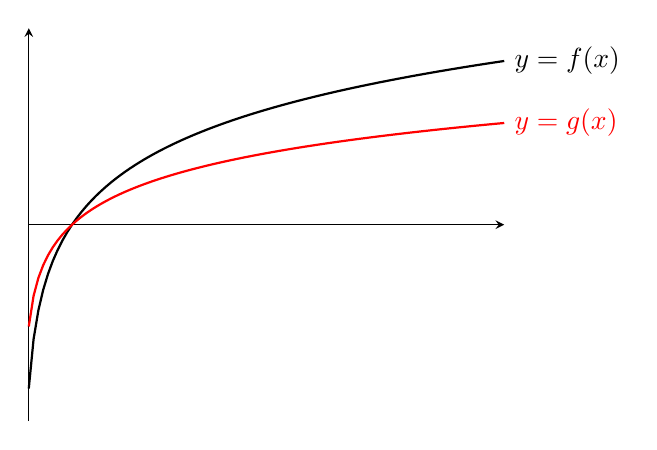
\begin{tikzpicture}
          \begin{axis}[xtick=\empty, ytick=\empty, clip=false]
            \addplot[domain=0:10] {ln(x)} node[right] {$y=f(x)$};
            \addplot[domain=0:10, red] {ln(x)/ln(5)} node[right] 
            {$y=g(x)$};
          \end{axis}
        \end{tikzpicture}
      \end{center}
    \end{solution}

  \item \label{sketch-deriv-of-ln}
    \begin{problem}[\vfill]
      In white chalk, sketch the graph of $f'(x)$. On the same set of axes, sketch the graph of $g'(x)$ in colored chalk.
    \end{problem}

    \begin{solution}
      \begin{center}
        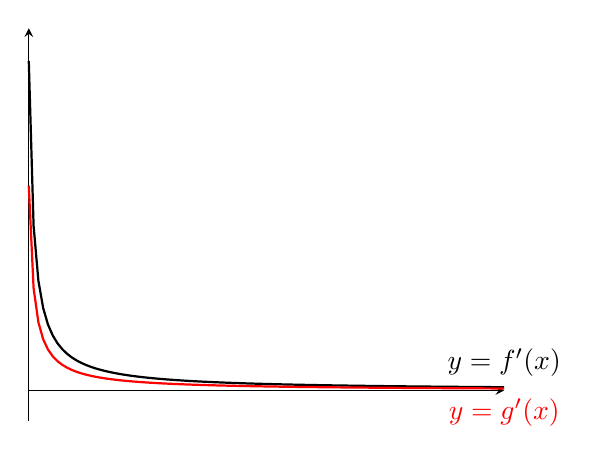
\begin{tikzpicture}
          \begin{axis}[xtick=\empty, ytick=\empty, clip=false]
            \addplot[domain=0:10] {1/x} node[above] {$y=f'(x)$};
            \addplot[domain=0:10, red] {1/(x*ln(5))} node[below]
            {$y=g'(x)$};
          \end{axis}
        \end{tikzpicture}
      \end{center}
    \end{solution}

  \item

    \note{Here, I want students to remember the meaning of $\ln 10$ as the power you must raise $e$ to in order to get 10. And this gives us a way to check which graph should be higher when $x = 10$.}

    \begin{problem}[\stretch{0.25}]
      Which is greater, $\ln 10$ or $\log_5 10$? Why?
    \end{problem}

    \begin{solution}
      Remember that $\ln 10$ is the power we raise $e$ to in order to get 10, and $\log_5 10$ is the power we raise $5$ to in order to get 10.

      Since $e < 5$, the power we need to raise $e$ to in order to get 10 is greater than the power we need to raise $5$ to in order to get 10. Therefore, $\ln 10 > \log_5 10$. 
    \end{solution}

  \item \label{derivative-of-log5}

    \note{Now, we'll remember that $\log_5 x$ is just a constant multiple of $\ln x$.}

    \begin{problem}[\stretch{0.5}]
      Use the change of base formula to express $g(x) = \log_5 x$ in terms of $f(x) = \ln x$. Is this consistent with your graphs? 
    \end{problem}

    \begin{solution}
      Using the change of base formula, $\log_5 x = \frac{\ln x}{\ln 5}$.
      Thus, $g(x) = \frac{1}{\ln 5} f(x)$. This is consistent
      with our graphs, which show that $y=g(x)$ is a vertical scaling
      of $y=f(x)$.
    \end{solution}

    \begin{problem}[\nstretch{0.1}]
      What does this tell you about how $g'(x)$ relates to $f'(x)$?
    \end{problem}

    \begin{solution}
      This tells us that $g'(x)=\frac{1}{\ln 5} f'(x)$.
    \end{solution}

  \end{enumerate}

\item  \label{derivative-of-ln-x}

  \note{In the previous problem, we saw that the derivative of $\log_5 x$ is just $\dfrac{1}{\ln 5} \dfrac{d}{dx} (\ln x)$. So, if we want to find derivatives of $\log_b x$ for any $b > 0$, we can just focus on finding the derivative of $\ln x$.}

  Let $f(x) = \ln x$. In this problem, we'll figure out a formula for $f'(a)$.

  \begin{enumerate}
  \item

    \note{I just want them to see that we don't get anywhere with this, since there's no way to simplify $\ln(a + h)$}

    \begin{problem}[0.5in]
      Write the limit definition of $f'(a)$.
    \end{problem}

    \begin{solution}
      \begin{align*}
        f'(a) &= \lim_{h \to 0} \frac{f(a+h)-f(a)}{h} \\
        &= \lim_{h \to 0} \frac{\ln(a+h) - \ln(a)}{h}
      \end{align*}
    \end{solution}

    \note{So, we need a different approach. It turns out that we can use the fact that $\ln x$ is the inverse function of $e^x$ (and we know the derivative of $e^x$) to find the derivative of $\ln x$.}

  \item

    \begin{problem}
      On the axes below, a value $a$ is marked. Sketch the graph of $f(x) = \ln x$ together with a line whose slope is $f'(a)$.
    \end{problem}

    \begin{problemonly}
      \axes[axis equal image, xtick={1, e}, xticklabels={1, $a$}, ytick=\empty, width=4in, enlarge y limits=false, xmin=-2, xmax={e^1.5}, ymin=-2, ymax={e^1.5}]
    \end{problemonly}

    \begin{solution}
      \begin{center}
        \begin{tikzpicture}
          \begin{axis}[axis equal image, xtick={1, e}, xticklabels={1, $a$}, ytick=\empty, width=3.5in, enlarge y limits=false, xmin=-2, xmax={e^1.5}, ymin=-2, ymax={e^1.5}]
            \addplot+[domain={1/e^2}:{e^1.5}] {ln(x)}; %
            \addplot+[closed] coordinates {(e, 1)} node[anchor=north west]{$(a, \ln a)$}; % 
            \addplot+[hotpink, domain={e-1.5}:{e+1.5}] {1/e*(x-e) + 1}; % 
          \end{axis}
        \end{tikzpicture}        
      \end{center}
    \end{solution}

  \item
    \begin{problem}
      On the picture above, sketch the reflection of both the curve and the line over $y = x$. 
    \end{problem}

    \begin{solution}
      \begin{center}
        \begin{tikzpicture}
          \begin{axis}[axis equal image, xtick={1, e}, xticklabels={1, $a$}, ytick=\empty, width=3.5in, enlarge y limits=false, xmin=-2, xmax={e^1.5}, ymin=-2, ymax={e^1.5}]
            \addplot+[domain={1/e^2}:{e^1.5}] {ln(x)}; %
            \addplot+[closed] coordinates {(e, 1)} node[anchor=north west]{$(a, \ln a)$}; % 
            \addplot+[hotpink, domain={e-1.5}:{e+1.5}] {1/e*(x-e) + 1}; %
            \addplot+[domain=-2:1.5, blue] {e^x}; %
            \addplot+[closed] coordinates {(1, e)} node[anchor=south east, fill=white] {$(\ln a, a)$}; %
            \addplot+[purple, domain={1-1.5/e}:{1+1.5/e}] {e*x}; %
            \addplot+[dashed, gray, domain=-2:{e^1.5}] {x}; %
          \end{axis}
        \end{tikzpicture}        
      \end{center}
    \end{solution}

  \item
    \begin{problem}[\vfill]
      Find the slope of the reflected line. (\emph{Hint:} What's the reflected function?) 
    \end{problem}

    \begin{solution}
      The blue curve is the graph of the inverse function of $f(x) = \ln x$, so it's the graph of $g(x) = e^x$. Therefore, the slope of the purple tangent line is $g'(\ln a)$, which we can calculate:
      \begin{align*}
        g'(x) &= e^x \\
        g'(\ln a) &= e^{\ln a} = a 
      \end{align*}
    \end{solution}

  \item
    \begin{problem}[\stretch{0.5}]
      What does that tell you about the slope of the original line?  
    \end{problem}

    \begin{solution}
      Since the pink line is the reflection of the purple one, its slope is $\dfrac{1}{a}$. So, $f'(a) = \dfrac{1}{a}$! 
    \end{solution}

  \item \label{deriv-of-ln}
    \begin{problem}[\nstretch{0.5}]
      What's $f'(x)$? Is this consistent with the graph you sketched in \ref{sketch-deriv-of-ln}? 
    \end{problem}

    \begin{solution}
      We determined $f'(a)=\frac{1}{a}$, so $f'(x)=\frac{1}{x}$. This
      matches the graph we sketched in \ref{sketch-deriv-of-ln}. 
      (The domain of $f'$ is $(0, \infty)$ because the domain of $f$
      is $(0, \infty)$.)
    \end{solution}
  \end{enumerate}

\item 

  \note{We've already seen that $\dfrac{d}{dx} \log_5 x = \dfrac{1}{\ln 5} \dfrac{d}{dx} (\ln x)$, but students will end up saying things like $\dfrac{1}{5x}$ here. Some may also try to use the Quotient Rule; if that comes up, it's worth talking about why that isn't necessary.}

  \begin{problem}[0.5in]
    Use \ref{derivative-of-log5} and \ref{deriv-of-ln} to find the derivative of $\log_5 x$.
  \end{problem}

  \begin{solution}
    We found in \ref{derivative-of-log5} that $\frac{d}{dx} \log_5 x = 
    \frac{1}{\ln 5} \frac{d}{dx} \ln x$. Therefore 
    $\frac{d}{dx} \log_5 x = 
    \frac{1}{\ln 5}(\frac{1}{x})$, or $\frac{1}{x \ln 5}$.
  \end{solution}

\end{enumerate}
\begin{framed}
  \emph{Derivatives we know.}
  \begin{multicols}{2}
    \begin{itemize}

    \item $\displaystyle \frac{d}{dx} (x^n) = \solonly{nx^{n-1}}$  
      $\qquad   \qquad $  ($n$ is a
      constant)
    \item $\displaystyle \frac{d}{dx} (e^x) = \solonly{e^x} \qquad   \qquad $  
    \item $\displaystyle \frac{d}{dx} (e^{kx}) = \solonly{ke^{kx}}  \qquad   \qquad $ ($k$ is
      a constant)

    \item $\displaystyle \frac{d}{dx} (b^x) = \solonly{b^x\ln b} \qquad \qquad $ ($b>0$ and
      constant)
    \item $\displaystyle \frac{d}{dx} (\ln x) = 
    \solonly{\frac{1}{x}}\qquad \qquad $
    \item $\displaystyle \frac{d}{dx} (\log_b x) = \solonly{\frac{1}{x\ln b}}\qquad $ ($b>0$
      and constant)

    \end{itemize}
  \end{multicols}  
\end{framed}

\begin{enumerate}[resume]
\item 
  \begin{problem}[1.25in]
    Write down the log rules we learned last time.
  \end{problem}

  \begin{solution}
    \begin{itemize}[topsep=0pt]
  \item \solonly{$\displaystyle \log_b (uw) = \log_b u + \log_b w$} \

  \item \solonly{$\displaystyle \log_b \left(\frac{u}{w}\right) = \log_b u - \log_b w$}\

  \item \solonly{$\displaystyle \log_b \left(u^n\right) = n \log_b u$}\

  \end{itemize}  
  \end{solution}

\item 

  Find the derivative of each of the following functions. You'll need to either use logarithm rules or exponential rules to rewrite the function in a form that you can differentiate, or take advantage of the Chain Rule and differentiate right away. Experiment with both! (If the Chain Rule feels overwhelming today, rest assured we'll be reviewing derivatives tomorrow.)

  \begin{enumerate}
  \item
    \begin{problem}[\vfill]
      $g(x) = \ln (3x^2)$
    \end{problem}

    \begin{solution}
      First, let's use log rules to rewrite $g(x)$ as 
      $g(x)=2\ln(x)+\ln(3)$. Then using our derivative rules,
      $g'(x)=\boxed{\frac{2}{x}}$.
    \end{solution}

  \item
    \begin{problem}[\vfill]
      $f(t) = \ln \left( e t^t \right)$
    \end{problem}

    \begin{solution}
      Using log rules, $f(t)=\ln(e) + t\ln t$. We need to use the
      Product Rule:
      $f'(t)=1\cdot\ln t + t \cdot \frac{1}{t} =\boxed{\ln t +1}$.
    \end{solution}

  \item
    \begin{problem}[\vfill\newpage]
      $j(x) = e^{3x - 2}$ (Hint: We know how to differentiate functions of the form $C e^{kx}$ or $C \cdot b^x$. Can you rewrite this in one of those two ways?) 
    \end{problem}

    \begin{solution}
      We can rewrite $j(x)$ as $j(x)=e^{-2}e^{3x}$. So
      $j'(x)=3e^{-2}e^{3x}=\boxed{3e^{3x-2}}$.
    \end{solution}

  \item
    \begin{problem}[\vfill]
      $\displaystyle y = \frac{\sqrt[3]{8 \cdot 5^x}}{7}$
    \end{problem}

    \begin{solution}
      First, let's rewrite $y$ as $y=\tfrac{2}{7} 5^{x/3}$. We
      can use exponent rules to further write $y=\tfrac{2}{7} (5^{1/3})^x$.
      Therefore $dy/dx = \boxed{\tfrac{2}{7} \ln(5^{1/3}) (5^{1/3})^x}$.
    \end{solution}

  \item
    \begin{problem}[\vfill]
      $g(x) = \log_2 \left( \dfrac{2^x}{\sqrt[3]{x}} \right)$
    \end{problem}

    \begin{solution}
      We can use log rules to write 
      $g(x) = \log_2 (2^x) - \log_2 \sqrt[3]{x} 
      = x - \tfrac{1}{3} \log_2 x$. Using our derivative rules,
      $g'(x) = \boxed{1-\frac{1}{3x\ln2}}$.
    \end{solution}

  \item
    \begin{problem}[\vfill]
      $h(x) = e^{-3 \ln x}$
    \end{problem}

    \begin{solution}
      First, we can rewrite $h(x)$ as $h(x) = e^{\ln(x^{-3}}=x^{-3}$.
      So $h'(x) = \boxed{-3x^{-4}}$.
    \end{solution}

  \item

    \begin{problem}[\vfill\newpage]
      $\displaystyle g(w) = \frac{\log_7(w)}{7^w}$
    \end{problem}

    \begin{solution}
      We can use the Quotient Rule. Optionally, we can try to simplify.
      \begin{align*}
          g'(w) &= \frac{\frac{1}{w\ln7}\cdot 7^w - 7^w\ln7 \log_7(w)}{(7^w)^2} \\
          &= \frac{\frac{1}{w\ln7}-\ln7 \log_7{w}}{7^w} \\
          &= \frac{1-(\ln 7)^2w\log_7 w}{7^w w \ln 7} \\
          &= \frac{1-(\ln 7)^2w\frac{\ln w}{\ln7}}{7^w w \ln 7} \\
          &= \boxed{\frac{1-(\ln7) w\ln w}{7^w w \ln 7}}
      \end{align*}
    \end{solution}

  \end{enumerate}

\item  

  Let $f(x) = x \ln \sqrt{x}$.
  \begin{enumerate}
  \item
    \begin{problem}[0.5in]
      What's the domain of $f$? 
    \end{problem}

    \begin{solution}
      We can't take the logarithm of a non-positive number, so the
      domain is $(0, \infty)$.
    \end{solution}

  \item

    \begin{problem}[\stretch{2}]
      Does $f(x) = x \ln \sqrt{x}$ have a global maximum on its domain? If so, where? How about a global minimum? 
    \end{problem}

    \begin{solution} 
      We don't know how to differentiate $\ln \sqrt{x}$, so let's first use logarithm rules to rewrite $\ln \sqrt{x} = \ln \left( x^{1/2} \right) = \frac{1}{2} \ln x$. So, $f(x) = \frac{1}{2} x \ln x$, and
      \begin{align*}
        f'(x) &= \frac{1}{2} \frac{d}{dx} (x \ln x) \text{ by the Constant Multiple Rule} \\
        &= \frac{1}{2} \left[ x \frac{d}{dx} (\ln x) + \left( \frac{d}{dx} x \right) \ln x \right] \text{ by the Product Rule} \\
        &= \frac{1}{2} \left[ x \cdot \frac{1}{x} + 1 \cdot \ln x \right] \\
        &= \frac{1}{2} \left( 1 + \ln x \right)
      \end{align*}
      This is defined on $(0, \infty)$, but it is 0 at $x = e^{-1}$. So, there is only one critical point, $\frac{1}{e}$.

      Since there's only one critical point, we can use the Second Derivative Test. We have
      \begin{align*}
        f''(x) &= \frac{1}{2} \cdot \frac{1}{x} = \frac{1}{2x} \\
        f'' \left( \frac{1}{e} \right) &= \frac{1}{\quad \frac{2}{e} \quad} > 0
      \end{align*}
      So, $\frac{1}{e}$ is a local minimum. Since it's the only critical point, $f$ has a \fbox{global minimum at $x = \frac{1}{e}$} and
      \fbox{no global maximum}.
    \end{solution}

  \end{enumerate}

\end{enumerate}
\end{document}
